\documentclass[a4paper,12pt]{article}
\usepackage{graphicx}  % 用于插入图片
\usepackage{geometry}  % 用于设置页面尺寸
\geometry{margin=1in}  % 设置边距为1英寸
\usepackage{titlesec}  % 用于设置标题样式
\usepackage{setspace}  % 用于设置行距
\usepackage{fancyhdr}  % 用于设置页眉页脚
\usepackage{pdfpages}  % 导入pdfpages宏包
\usepackage{hyperref}
\usepackage{csquotes} 

% 设置行距
\onehalfspacing

% 设置页眉页脚
\pagestyle{fancy}
\fancyhf{}
\rfoot{\thepage}

% 设置标题格式
\titleformat{\section}{\large\bfseries}{\thesection}{1em}{}

% 封面
\begin{document}
\begin{flushright}
    ISYS2120 Sem2, 2024
\end{flushright}

\vspace{2cm}

\begin{center}
    \Huge \textbf{Assignment 2 Individual Report}
\end{center}

\vspace{2cm}

\noindent
\textbf{SID:}

\vspace{1cm}

\begin{center}
    \fbox{
        \parbox{10cm}{
            \vspace{1cm}
            \hspace{3cm}\texttt{530157791}
            \vspace{1cm}
        }
    }
\end{center}

\vspace{2cm}

\begin{center}
    \textit{(Do not edit the format of this cover sheet!)}
\end{center}

\newpage
% Part A: ER图
\section*{Part A: Extended ER Diagram}
\noindent
This section contains the extended ER diagram. Here are links to \hyperlink{PartB}{Part B} and \hyperlink{PartC}{Part C}

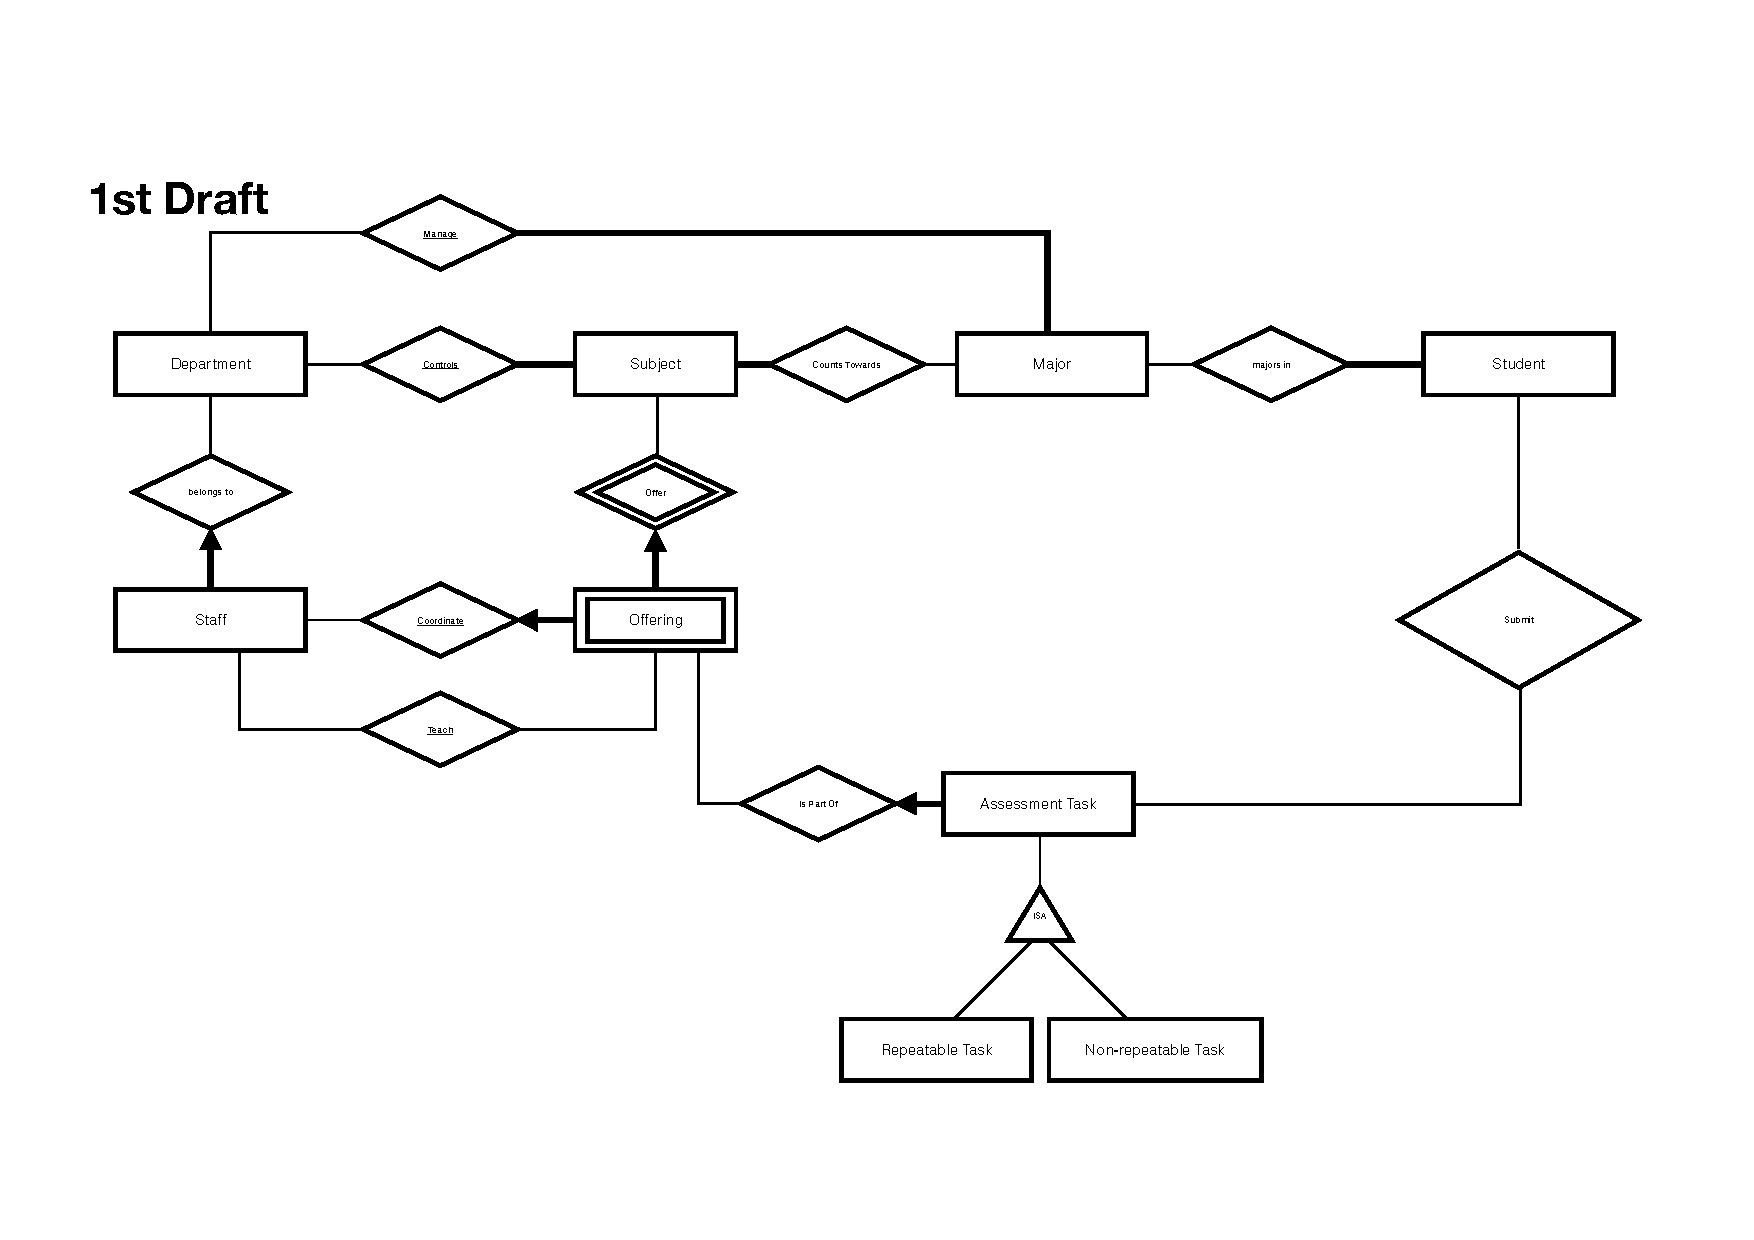
\includepdf[pages={1-6}]{Graphs/ER-diagram.pdf}

\newpage

% Part B: 检查过程描述
\section*{Part B: Diagram Validation and Checking Process}
\hypertarget{PartB}{}
\noindent

\subsection*{Checking}
In this section, I describe how I checked the ER diagram for validity and correctness based on the system's textual description. The following checks were performed:

\begin{itemize}
  \item \texttt{The system needs to keep a scan of every submission made by a student for an assessment task.A submission is handed in at a date and time which must be recorded, and it may have been awarded a mark by a staff member.}

  This sentence indicates a many to many relationship from student to assessment task with attributes \texttt{date}, \texttt{time} and \texttt{mark}. This is because each student can submit assignments for multiple assessment tasks, and each assessment task can also have submissions from multiple students. According to Ed post \texttt{\#497}, we should also record which \texttt{staff} marked this submission. However, this information cannot be represented in the current ER diagram.

  \item \texttt{The system needs to keep information for each student, including their studentkey (an identifier such as JS2X57), surname, given name, year-of-entry, major(s), official email, and address}

  For this description, we can model \texttt{Student} as an entity set with attributes including \texttt{studentkey, surname, given name, year-of-entry, major(s), official email,} and \texttt{address}. However, considering \texttt{major} as an entity set, modeling it as an attribute under \texttt{Student} does not accurately represent the many-to-many relationship between \texttt{Student} and \texttt{Major}.

  In the ER diagram, the \texttt{Student} entity correctly includes \texttt{studentkey (PK)} and the other attributes mentioned above except for \texttt{major}. It also depicts the many-to-many relationship between \texttt{Student} and \texttt{Major}, with total participation of \texttt{Student}, accurately reflecting that each student belongs to at least one major, and each major can have multiple students.

  \item \texttt{Staff members are identified by staffId, and have surname, given name, title, department, official email, and contact phone number. }

  Based on the description, we need to introduce \texttt{Staff} as an entity set, with attributes including \texttt{surname, given name, title, department, official email}, and \texttt{contact phone number}.

  The ER diagram does show the \texttt{Staff} entity and its attributes.

  \item \texttt{Each assessment task occurs for an offering of a subject [for example, the offering of the subject Traditional Philosophy in sem1 of 2024], and the assessment task has a name (eg “Assignment 1”), a weight towards the grade in the offering, a kind (such as Essay, Quiz, ProblemSet, FinalExam), an instruction document, and a latest-date-for-submission.}

  The sentences describe an entity set \texttt{Assessment Task} with the attributes: \texttt{Name, Weight, Kind, LatestDate}, and \texttt{Instruction Document}. Since each \texttt{Assessment Task} must belong to a specific \texttt{Offering}, and an Assessment Task cannot be distinguished based on its own attributes, different assessments across different offerings may have the same attributes. Therefore, \texttt{Assessment} should be considered a Weak Entity that depends on \texttt{Offering}.

  In addition, \texttt{Offering}, as an entity set, needs to be identified through \texttt{Subject, year, and semester} (according to Ed post \#399). This indicates that \texttt{Offering} is a Weak Entity Set, where both \texttt{year} and \texttt{semester} are distinguishing attributes.

  In the current diagram, \texttt{Offering} is represented as a Weak Entity, but \texttt{Assessment Task} is depicted as a regular entity, with an added Assessment ID as the primary key. This needs to be reconsidered. The current diagram does not represent \texttt{Assessment} as a Weak Entity.

  \item \texttt{Some assessment tasks are non-repeatable; this means that a student may not submit for this more than once, and in that case, there is a mechanism for the student to request an exemption for illness (the system needs to track the text of the request, the date it was made, and whether or not this was approved). For an assessment which does allow multiple submissions, we need to keep information on a policy which decides how to calculate the overall score the student gets (for example, it may be that only the latest submission is marked, or that each submission is marked and the highest mark is used, or maybe the latest submission is marked but a penalty is subtracted based on the number of submissions made). }

  The description explains that assessment tasks can be divided into two categories: repeatable and non-repeatable, each with different attributes that need to be recorded. For non-repeatable tasks, the system needs to track whether a student has requested an exemption due to illness, including recording the request text, submission date, and whether the request was approved, as well as defining the relationship between the student and the exemption. For tasks that allow multiple submissions, the system needs to store a grading policy. The current ER diagram uses the ISA structure to represent these two types of assessment tasks. Common attributes such as task name, weight, and type are stored in the parent class, Assessment Task, while specific attributes are stored in their respective subclasses:

  \begin{itemize}
    \item For non-repeatable tasks, information related to exemption requests is stored, including the request text, submission date, and approval status.

    \item For repeatable tasks, the grading policy is stored. The design in the diagram correctly captures these relationships and clearly distinguishes the two types of tasks through the ISA structure. However, the diagram does not represent the relationship between the student and the exemption request.
  \end{itemize}


  \item \texttt{For a subject, we need to know its name, the credit-hours it carries, the major(s) it counts towards [if any], and whether or not students are allowed to take it more than once.}

  This statement clearly indicates that \texttt{Subject} should be represented as an entity set, and its attributes should include the \texttt{name, credit hours, and whether it allows retaking}. Additionally, each subject may be associated with zero or more majors,indicating a many-to-many relationship between \texttt{Subject} and \texttt{Major}. However, there are two errors in the diagram: First, the relationship between \texttt{Subject} and \texttt{Major} is incorrectly depicted as requiring all subjects to participate in this relationship, when in reality, a subject may not belong to any major. Second, the \texttt{Subject} entity should not have multi-valued attributes, as this aspect is already captured by the relationship.

  \item \texttt{The same subject may be taught over several offerings and the assessment tasks will be different between these offerings (though they may share a name!)}

  This statement clarifies that the relationship from \texttt{Subject} to \texttt{Offering} should be one-to-many, with all \texttt{Offerings} participating in this relationship. Additionally, the relationship between \texttt{Assessment Task} and \texttt{Offering} should be many-to-one, with all Assessment Tasks required to participate. 

  These relationships are clearly represented in the diagram using bold arrows. Considering that Assessment Tasks may have the same name, the diagram introduce an attribute \texttt{AssessmentID} to distinguish between them.

  \item \texttt{Each offering is taught by a staff member as coordinator, and possibly there are other staff as teachers as well. }

  In this description, we can identify two distinct relationships between Staff and Offering:
  \begin{enumerate}
    \item A many-to-one relationship from \texttt{Offering} to \texttt{Staff}, where every Offering is associated with exactly one coordinator. This means that each \texttt{Offering} has exactly one coordinator.

    \item A many-to-many relationship, indicating that an \texttt{Offering} can be taught by multiple Staff members, and a single Staff member can teach multiple Offerings.
  \end{enumerate}

  The current diagram accurately represents both of these relationships.


  \item \texttt{The staff are each members of a department, and every subject is under control of some department.}

  The description reflects two relationships:
    \begin{enumerate}
        \item Staff should belong to a department, but due to the unclear phrasing, the specific type of relationship in the diagram is still ambiguous.

        \item Every subject should be controlled by a department, but the description does not specify whether it can be controlled by multiple departments.
    \end{enumerate}

  The relationships depicted in the current diagram may not cover all potential cases, and further discussion is required.

  \item \texttt{A department may be responsible for a major (and indeed, some majors may be shared between departments, eg “Greek History” major is shared between Classics department and History department).}

  A many-to-many relationship from department to major is reflected in this statement. However, since it does not clearly specify whether all majors must be managed by a department, the specific details of the relationship remain unclear. The diagram currently assumes that all majors must be part of the relationship.


\end{itemize}

\subsection*{Strength}
    \begin{enumerate}
        \item The ER diagram uses a weak entity to reflect the fact that \texttt{Offering} cannot be distinguished by its own attributes. This design accurately describes that \texttt{Offering} can only be identified through the combination of \texttt{semester, year, and subject}. When converting to a relational schema, the relationship between \texttt{Subject} and \texttt{Offering} becomes easier to understand.

        \item Through the ISA structure, the ER diagram accurately distinguishes between repeatable and non-repeatable tasks while sharing common attributes in the parent entity, thus avoiding redundant design. 

    \end{enumerate}

\subsection*{Limitation}
    \begin{enumerate}
        \item In the current diagram, although the \texttt{mark} of a submission can be recorded as an attribute of the submit relationship, the current diagram is unable to capture which staff member marked each submission.
        
        \item The relationship between \texttt{Staff} and \texttt{Department} in the diagram shows that each staff member must belong to only one department. However, this design may not be sufficient to capture all possible scenarios, as staff members could also belong to multiple departments.

        \item For the \texttt{Subject} entity set, the implementation of the \texttt{major} information is duplicated: it is represented both as a multi-valued attribute in \texttt{Subject} and through the relationship between \texttt{Subject} and \texttt{Major}. This design is unclear and confusing.

        \item For a Non-repeatable Task, in the current ER diagram, at the conceptual model level, there is no restriction that an Assessment without exemptions can only be submitted once. In the current design, regardless of whether it is repeatable or non-repeatable, there is no limitation on the number of submissions shown in the diagram.

        \item In the current design, \texttt{exemption} is an attribute of a \texttt{Non-Repeatable Task}. This design has two issues: 
        \begin{itemize}
            \item we are currently unable to record which student submitted the exemption. 
            \item In the current design, a Non-Repeatable Task can only have one exemption, but in reality, multiple students may apply for an exemption for the same Non-Repeatable Task.
        \end{itemize}

    \end{enumerate}

\subsection*{Suggestion}
    \begin{enumerate}
        \item To record which staff member graded a submission, we could consider modeling submission as an entity set instead of a relationship. In this approach, the relationships between \texttt{Assessment Task, Student, Staff,} and \texttt{Submission} can be more precisely defined.
        
        \item The relationship between Staff and Department should be clarified. We should \texttt{check} Ed for any relevant definitions, and if none are provided, we can make assumptions based on real-world scenarios.

        \item When representing the majors a Subject belongs to, it should be decided whether to capture this information using an attribute or a relationship. The decision on which to keep should be based on the clarity of the ER diagram and the ease of implementation.

        \item Non-repeatable Task: Attempt to clarify the definition of exemption and see if adding an extra submission will be allowed. Additionally, try to implement a constraint: Assessments without exemption can only be submitted once.

        \item The names of the relationships need to be reconsidered, using single verbs that are as easy to understand as possible.

    \end{enumerate}

\newpage

\section*{Part C: Group Process Description}
\hypertarget{PartC}{}
\noindent
\subsection*{Design Process}
In this assignment, our group members independently completed all sections and then compared two different versions, integrating the best design. Below are the meeting times and records:

\begin{table}[h!]
\centering
\begin{tabular}{|c|c|p{10cm}|}
\hline
\textbf{Date} & \textbf{Location}    & \textbf{Meeting Notes}                                                                                                    \\ \hline
9/2           & Glebe                & Discussed assessment requirements and planned the conceptual model and report submission. Decided on independent work for all parts before integration. \\ \hline
9/6           & Tutorial consultation & Discussed unclear points and confirmed requirements with tutor.                                                           \\ \hline
9/9           & Fisher Library        & Compared each member’s versions, merged into the draft final version, and assigned report writing tasks.                   \\ \hline
\end{tabular}
\end{table}

When deciding on the final ER diagram, we first compared the differences between the two versions and checked for any obvious logical errors, such as incorrect relationship types. If, for a particular part, we determined that both designs could correctly reflect the information, we chose the clearer design. Finally, we reviewed the requirements again to ensure that we hadn't missed any information.


\subsection*{Conflicts Resolution}

During our discussion, we had differing opinions on the design of Repeatable and Non-repeatable Tasks. The first approach stores all possible attributes in the Assessment Task entity and adding an new attribute to indicate whether it is repeatable or non-repeatable. The second approach proposed using an ISA structure, creating two new entity sets, with common attributes stored in the Assessment Task and specific attributes stored in the subclasses. We discussed the pros and cons of both structures. Although the first approach is simpler, it requires application-level constraints to determine whether certain attributes can store values, and storing the specific attributes of both types of tasks in the same table is not logically correct. In the end, we realized that these two types of assessments need to store different attributes, such as policies and exemptions, but they still share some common attributes. Therefore, we concluded that using the ISA structure is the most appropriate solution.

\subsection*{Effective Aspects}

Having each member complete all parts of the assignment allowed everyone to have a comprehensive understanding of the entire assignment. For each section, the different versions helped cover as much information as possible, improving the accuracy of the design and preventing errors that might arise from one person overlooking something. With everyone having a individual understanding of the entire assignment, group discussions became more meaningful, as all members were familiar with every part of the model, making it easier to identify potential issues.

\subsection*{Ineffective Aspects}

Since each member had to complete their own version first, this extended the design phase. When it came time to merge the final version, each person had more parts to review, which made the overall process longer.Additionally, we didn’t set clear goals for each stage, which led to inconsistent progress when trying to move to the next step, further reducing efficiency.

\subsection*{Suggestions for improvement}

In future projects, to improve efficiency, we can collaborate by dividing tasks based on each member's strengths rather than having everyone complete everything independently and then merge the results. At each stage, we should set clear objectives and allow some buffer time to handle any unforeseen issues. Additionally, team members should evaluate each other’s work and provide feedback for improvement throughout the process.


\end{document}

